\section{研究動機}
隨著科技的發展,我們越來越期望機器能夠理解問題並給予答案,進而解決一些生活上的事情。因此,我們需要一套問答系統(Question Answering System)來幫助我們快速的瀏覽資訊,並從中獲取答案。在過去有許多幫助我們回答問題,被開發出來並應用於產業中,如 Google Home(圖 \ref{fig:home_banner})、 Wolfram Alpha 、 Apple Siri 、 Amazon Alexa 等等。

\begin{figure}
    \centering
    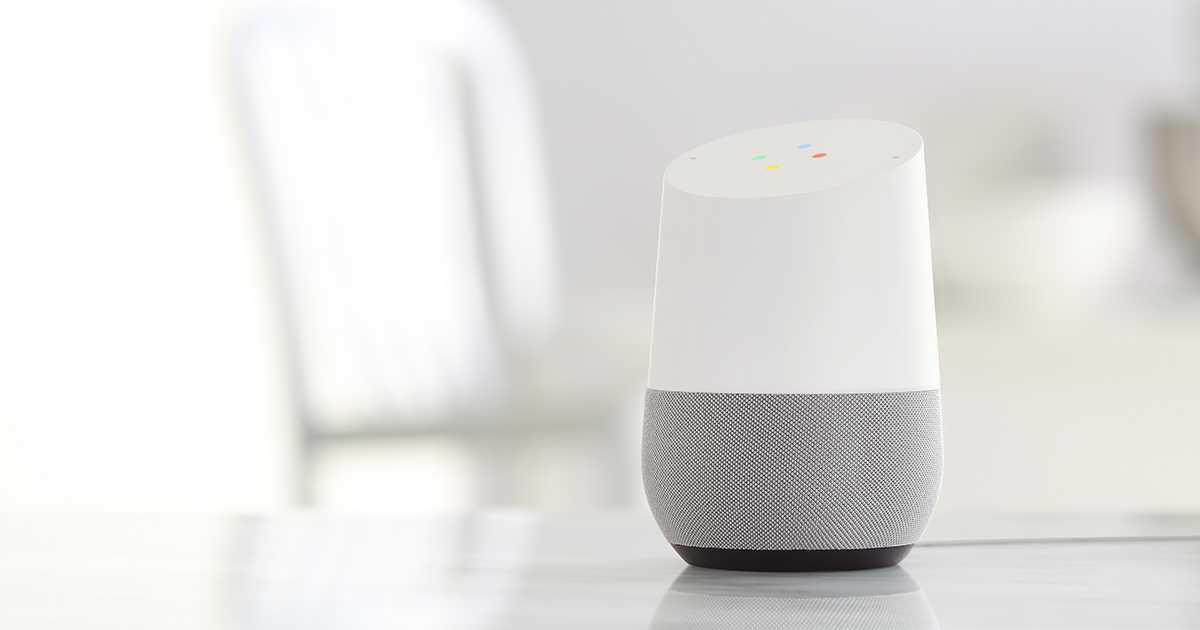
\includegraphics[scale=0.35]{images/home_banner.jpg}
    \caption{Google Home}\label{fig:home_banner}
\end{figure}

近年來隨著科技與網際網路的興起,維基百科(Wikipedia)等參考工具書正蓬勃地增加,人們追求更加直覺、便捷、有效率的資訊獲得途徑。在資料量大增的情況下,問答系統從大量的資料中直接擷取使用者想要的答案,僅只提供給使用者問題相關的答案,更加速了使用者獲得資訊的效率,因此如何讓機器能夠這些資料、理解、並回答問題,省去人們需要閱讀的時間,變成為重要的議題,而這即為問答系統。相較於其他的自然語言處理(Natural Language Processing)是提供給使用者文章、資源等,而問答系統有更困難的挑戰,如知識庫的廣大等,使得此問題更形艱辛。

近幾年更由於智慧型手機、穿戴式裝置的崛起與使用者需要在這些裝置上取得資訊的強烈需求,促使許多科技公司投入相關的研究,如 Facebook 有自己製造了如 bAbi 的人造資料集,希望機器在簡單的資料集上能有嬰兒一般學習能力、Google 整理了 CNN 以及每日郵報(Daily Mail)的新聞,以及 Microsoft 提供 MARCO 的資料集等,為的就是希望能在問答系統這塊能有顯著的突破。

而問答系統需要結合許多自然語言處理技術,如自然語言剖析(Natural Language Parsing)、問題分類(Question Classification)、專有名詞辨識(Named Entity Recognition)等等,另外少數問答系統會使用更複雜的邏輯推理機制,來區隔出需要推理機制才能夠區隔出來的答案。截至目前為止,最著名的問答系統應屬 IBM 在 DeepQA Project 中的超級電腦華生(Waston),並在 2011 年於 Jeopardy 節目中,與人類同場較勁,並獲得最後的勝利。

問答系統可以想像成複雜的自然語言處理問題,需要理解文字的意思。基本上,大多數(並非全部)的自然語言處理問題都能推廣成問答的問題,如機器翻譯(Machine Translation),可以對應成我們對此句話提問「此中文翻譯成英文是什麼」,因此我們若是能有好的問答系統模型架構,或許可以快速移植到自然語言處理的其他領域。
%TODO

% 相較於資訊檢索系統,是提供給使用者文章、資源等,而問答系統
\section{相關研究}%
問答系統是未來自然語言處理的明日之星,但也相當有難度。在過去的自然語言處理問題,往往是經過許多語言學家的多年的分析,如詞性標註(Part of Speech Tagging, POS Tagging)、專有名詞辨識、句法解析(Syntactic Parsing)、依賴關係解析(Dependency Parsing)、或是語言模型(Language Model)等等。近年來,專家們致力於研究出能夠自動化的解決自然語言處理領域的方法。在 2013 年由米氏 (Tomas Mikolov) 提出了方法,能夠有效的把文字投影到一向量空間(Vector Space),得到好的文字向量(Word Representations)\cite{mikolov2013efficient},使得在此之後,深度學習被廣泛地套用在自然語言處理領域,自然語言處理領域突飛猛進,研究者們紛紛踏入深度學習領域,試圖找尋更潛在的隱藏層(Hidden Layer),甚至深度學習的方法去取代過去自然語言處理的方法,試圖降低基於規則(Rule-Based)的依賴。

深度學習的架構非常多元,大多是以類神經網路為基礎延伸而成,有能夠抓取圖像中空間頻率的卷積類神經網路(Convolutional Neural Network, CNN)\cite{lecun1995convolutional}\cite{jia2014caffe}、能夠抓取短期時間資訊的遞迴式類神經網路(Recurrent Neural Network, RNN)\cite{mikolov2010recurrent}、利用閘道存取長時間時間資訊的長短期記憶神經網路(Long Short-term Memory Network, LSTM)\cite{hochreiter1997long} 等等。

\section{研究方向}
本論文之研究方向在探討以深度學習建立的問答系統模型,主要包含以下幾點:
\itemsep -2pt
\begin{itemize}
    \item 第一階段假想在少量文本並有包含符合問句的答案,進而生成出適當的句子來回答問句。
    \item 第二階段則探討如何在多個文本中,搜尋哪些文本包含有問句答案的文本。
    \item 第三階段探討基於搜尋出來的相關文本而生成出的句子,與原先已知相關文本產生句子,兩者之間的差距。
\end{itemize}
%本論文之目標在於閱讀文章的語意,並根據使用者的問句,試著去回答出答案,讓使用者更快速方便地獲得資訊,主要研究方向如下。
%\begin{itemize}
%    \item 傳統的自然語言處理需要對語言學有相關的知識,經過依賴關係解析(Dependency Parsing)和詞性標註(Part of Speech Tagging, POS Tagging)來分析句子的結構,並找出問句與文章之間的相關性。而深層類神經網路有好的推廣性,能省去其背後的分析,並且亦能有效的排除雜訊。
%    \item 再者,為了能夠將字與字和句與句前後關係連結起來,採用位置編碼(Position Encoding)和時間遞歸神經網路(Recurrent neural network)中的閘門遞迴單元來產生一個句子的向量表示(Vector Representation)。
%    \item 由於有些句子可能是跟問題句子無關的,我們採用了專注式模型(Attention Mechanism)來找尋出重要的句子,忽視與問句無關的句子,藉此模擬人們的專注力。
%    \item 藉由問句所通過編碼器的隱藏狀態(hidden state)當成記憶(Memory),並靠著文章的向量表示來多次更新記憶。
%    \item 最後以記憶當成解碼器的初始狀態,試著產生符合問句以及文章的句子。其中為了避免過度貼近(Overfit)測試資料,採用了權重遞減(l2 regularization)以及丟棄法(Dropout)。
%\end{itemize}

\section{章節安排}
本論文之章節安排如下:
\begin{itemize}
\itemsep -2pt
    \item 第二章:介紹本論文相關背景知識:包含深度類神經網路、時間遞歸神經網路、文字向量(word2vec)等等。
    \item 第三章:介紹如何以專注記憶式解碼器產生答案。
    \item 第四章:介紹如何檢索出包含有問句答案的文本。
    \item 第五章:介紹在基於檢索出的文本與已提供的相關文本所產生句子之差異。
    \item 第六章:本論文之結論與未來研究方向。
    %\item 第三章:介紹如何以專注記憶式網路選擇適當的答案。
\end{itemize}
